\documentclass[tikz,border=3pt]{standalone}
\usepackage[utf8]{inputenc}
\usepackage[T1]{fontenc}
\usepackage{lmodern}
\renewcommand{\familydefault}{\sfdefault}
\usepackage{sansmath}\sansmath
\usepackage{pgfplots}\pgfplotsset{compat=1.18,/pgf/number format/use comma,/pgf/number format/1000 sep={.}}
\usetikzlibrary{arrows.meta,calc,positioning,decorations.pathmorphing,patterns}
% paleta del sitio
\definecolor{nar}{HTML}{E8680C}\definecolor{narc}{HTML}{FFB35C}\definecolor{hielo}{HTML}{FFF3E8}
\definecolor{tinta}{HTML}{1D1D1F}\definecolor{gris}{HTML}{6E6E73}\definecolor{lila}{HTML}{7C5CF0}
\definecolor{azul}{HTML}{2F6FD6}\definecolor{menta}{HTML}{17A673}\definecolor{coral}{HTML}{E8342A}
\begin{document}
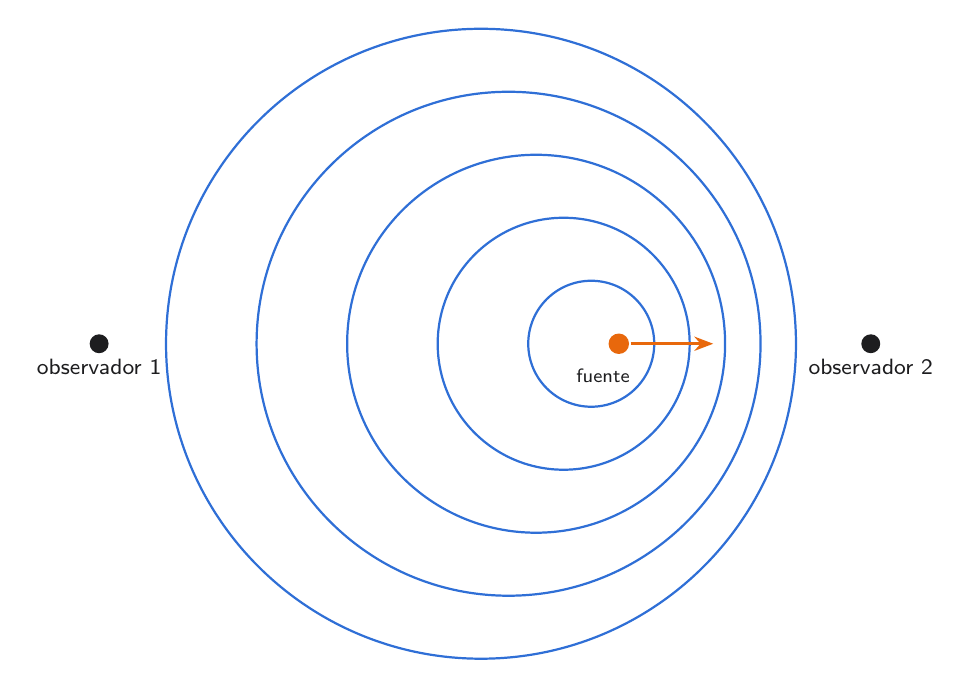
\begin{tikzpicture}[font=\footnotesize,>={Stealth[length=2.4mm]}]
\foreach \k in {1,...,5} \draw[azul,thick] ({-0.35*\k},0) circle ({0.8*\k});
\fill[nar] (0,0) circle (0.13);
\draw[->,very thick,nar] (0.15,0) -- (1.2,0);
\node[below,text=tinta,font=\scriptsize] at (-0.2,-0.2) {fuente};
\fill[tinta] (-6.6,0) circle (0.12) node[below=2pt] {observador 1};
\fill[tinta] (3.2,0) circle (0.12) node[below=2pt] {observador 2};
\end{tikzpicture}
\end{document}
